\documentclass[12pt, twocolumn]{article}
\usepackage[utf8]{inputenc}
\usepackage[spanish]{babel}
\usepackage{geometry}
\geometry{a4paper,margin=0.8in}
\usepackage{amsmath}
\usepackage{listings}
\usepackage{graphicx}
\usepackage{float}
\usepackage{url}
\usepackage{booktabs}
\usepackage{chngcntr}
\usepackage{amsfonts}
\usepackage{fancyhdr}
\pagestyle{fancy}
\cfoot{Página \thepage}
\counterwithin*{equation}{subsection}

\begin{document}
	\title{Medición del ritmo cardíaco por medios ópticos\\ 
		   \large{\textsc{Métodos Numéricos Avanzados}} \\
		   \normalsize{\textsc{Instituto Tecnológico de Buenos Aires}}}
	\author{
		\textsc{Balaguer}, Pedro \\
		\texttt{55795}
		\and
		\textsc{Benítez}, Julián \\
		\texttt{56283}
		\and
		\textsc{Garrigó}, Mariano \\
		\texttt{54393}
		\and
		\textsc{Perazzo}, Matías \\
		\texttt{55024}
		\and
		\textsc{Saqués}, M. Alejo \\
		\texttt{56047} 
	}
	\date{}
	\maketitle
	
	\begin{abstract}

	\end{abstract}
	
	\paragraph{Palabras clave:}
	
	\section{Resultados}
	
	\paragraph{} A continuación, se exhibirán los tiempos de ejecución entre las diferentes implementaciones del algoritmo \textit{fft} realizadas, como así también de los resultados obtenidos a la hora de calcular el ritmo cardíaco de un individuo.
	
	\subsection{Algoritmos \textit{fft}}
	
	\paragraph{} A continuación, se presenta una tabla comparativa de tiempos de ejecución entre la implementación recursiva e iterativa del algoritmo \textit{fft Cooley-Tukey}.
	
	\begin{table}[H]
		\centering
		\begin{tabular}{@{}llll@{}}
			\toprule
			N    & Recursivo & Iterativo & Mejora \\ \midrule
			512  & .009      & .003      & x3     \\
			1024 & .02       & .006      & x3.34  \\
			2048 & .046      & .014      & x3.29  \\
			4096 & .096      & .029      & x3.21  \\
			8192 & .201      & .06       & x3.35  \\ \bottomrule
		\end{tabular}
		\caption{Comparación entre implementaciones de \textit{Cooley-Tukey}}
		\label{fftcmp}
	\end{table}
	
	\paragraph{} Como podrá verse en la Tabla \ref{fftcmp}, la implementación iterativa del algoritmo \textit{Cooley-Tukey} es claramente del mismo orden algorítmico, pero en torno a $3.3$ veces más rápido. Se arguye que la mejora en la \textit{performance} proviene de la eliminación del \textit{overhead} generado por los \textit{stackframes} generados por la implementación recursiva en cada llamada.
	
	
	\subsection{Mediciones del ritmo cardíaco}
	
	\paragraph{} Se han tomado 5 muestras de un individuo en diferentes partes del cuerpo, variando el uso del \textbf{LED} del dispositivo:
	
	\begin{enumerate}
		\item Índice izquierdo $($cubriendo el \textbf{LED} con el mismo$)$,
		\item Pulgar derecho $($sin cubrir el \textbf{LED}$)$,
		\item Antebrazo,
		\item Índice derecho $($sin cubrir el \textbf{LED}$)$,
		\item Índice derecho $($con el \textbf{LED} apagado$)$.
	\end{enumerate}
	
	\paragraph{} Al momento de tomar las capturas, el individuo se encontraba en reposo. Se procuró que el mismo realizara inhalaciones y exhalaciones a intervalos regulares de aproximadamente 2 segundos, instruyéndole que realizara las mismas de manera calma.
	
	\paragraph{} A modo de control, se tomó una serie de muestras del ritmo cardíaco del individuo con mecanismos tradicionales. Para mayor precisión, se utilizó un estetoscopio y se contó durante el lapso de 1 minuto la cantidad de pulsaciones. Los siguientes parámetros describen la muestra:
	
	\begin{itemize}
		\item $N = 14$
		\item $\bar{X} = 78.929$
		\item $\sigma = 4.0089$
	\end{itemize}
	
	\paragraph{} A continuación se exhibirán los resultados utilizando diferentes métodos para obtener un valor escalar que represente el \textit{brillo} de la imagen para un instante dado, tomando una trama en escala de grises. 
	
	\paragraph{} Debe notarse que, en el análisis a continuación, se asume que el rimo cardíaco real permanece constante entre cada una de las muestras tomadas. Dadas las circunstancias en las que se re han realizado las mediciones, esta asunción puede tener un grado alto de validez. Sin embargo, eventuales variaciones podrían influir sobre la precisión de los errores presentados a continuación.
	
	\subsection{Región cuadrada con vértice en el centro}
	
	\paragraph{} Para este caso, se ha tomado una región cuadrada de $30X30$ con vértice en el centro de la imagen. Este caso es el utilizado por la Cátedra en el código de ejemplo.
	
	\begin{table}[H]
		\centering
		\begin{tabular}{@{}lll@{}}
			\toprule
			Muestra & Ppm.   & $|Error|$  \\ \midrule
			1    & 73.815 & 6.93\% \\
			2    & 75.592 & 4.41\% \\
			\textbf{3}    & 86.150 & 9.15\% \\
			4    & 80.854 & 2.44\% \\
			5    & 84.316 & 6.83\% \\ \bottomrule
		\end{tabular}
		\caption{Región $30X30$ con vértice en el centro}
		\label{3030}
	\end{table}
	
	\paragraph{} Como podrá verse en el Cuadro \ref{3030}, la aproximación con menor error relativo al promedio ha sido la de la muestra correspondiendo al dedo índice sin cubrir el \textbf{LED}. 
	
	\subsection{Promedio de toda la imagen}
	
	\paragraph{} En este caso, se han promediado todos los puntos de la imagen en escala de grises.
	
	\begin{table}[H]
		\centering
		\label{my-label}
		\begin{tabular}{@{}lll@{}}
			\toprule
			Muestra & Ppm.   &  $|Error|$    \\ \midrule
			1    & 73.815 & 6.93\%  \\
			2    & 86.139 & 9.13\%  \\
			3    & 87.908 & 11.38\% \\
			4    & 80.853 & 2.44\%  \\
			5    & 59.724 & 32.16\% \\ \bottomrule
		\end{tabular}
		\caption{Promedio de toda la imagen}
		\label{prom}
	\end{table}
	
	\paragraph{} Utilizando el método anterior, el error relativo en la muestra 5 era comparable al de las otras muestras. En el Cuadro \ref{prom}, podrá verse que dicho error, con este método, excede con creces el de las otras muestras. Esto indicaría que utilizar el \textbf{LED} podría ser un requisito no omisible a la hora de aproximar el ritmo cardíaco.
	
	\begin{figure}[H]
		\centering
		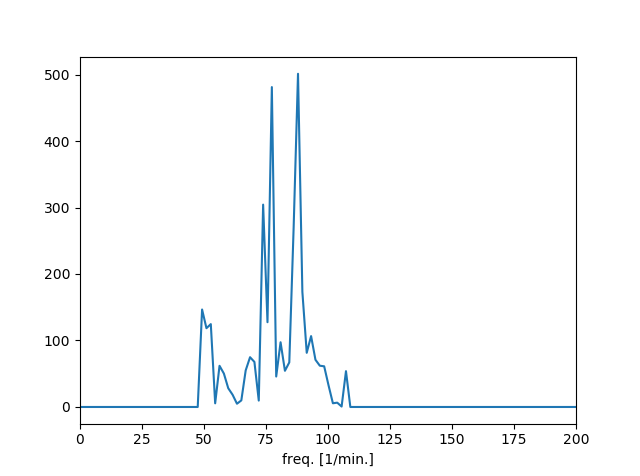
\includegraphics[width=8cm]{sample3_all.png}
		\caption{Muestra 3: proximidad entre picos}
		\label{3prox}
	\end{figure}
	
	\paragraph{} Otro caso cuyo error creció con respecto al obtenido en el método anterior es el de la muestra 3. Sin embargo, como se podrá ver en la Figura \ref{3prox}, existen dos picos de magnitud comparable claramente distinguibles uno del otro. El mayor es, razonablemente, el que corresponde a la frecuencia $87.908$. El que le sigue, corresponde al valor de $77.016$, lo que, de tomarse como valor del ritmo cardíaco, marcaría un $|Error| = 2.48\%$. Esto podría ser absolutamente azaroso, pero la eventual precisión del segundo valor en magnitud suscita curiosidad sobre la perspectiva de poder tomar la frecuencia del segundo mayor pico al tomar la medición en el antebrazo.
	
	\subsection{Región cuadrada con vértice en el centro, interpolando puntos}
	
	\paragraph{} Para este último caso, se ha tomado una región cuadrada de $200X200$ con vértice en el centro de la imagen, interpolando de a $5$ píxeles. El objetivo de esto es maximizar la superficie cubierta tomando una cantidad similar de píxeles que en el primer caso. Dado que se está filmando con la lente inmediatamente sobre la piel, la distancia real entre los píxeles es ínfima. Luego, interpolar muy probablemente de una aproximación cercana al verdadero promedio de todos los píxeles de la región.
	
	\begin{table}[H]
		\centering
		\begin{tabular}{@{}lll@{}}
			\toprule
			Muestra & Ppm.   &  $|Error|$   \\ \midrule
			1       & 73.815 & 6.93\%  \\
			2       & 73.834 & 6.90\%  \\
			3       & 87.908 & 11.38\% \\
			4       & 80.853 & 2.44\%  \\
			5       & 59.724 & 32.16\% \\ \bottomrule
		\end{tabular}
		\caption{Interpolando}
		\label{inter}
	\end{table}
	
	\paragraph{} Como podrá verse en la Tabla \ref{inter}, salvo una aparente mejoría en la muestra 2, los valores del $|Error|$ son aproximadamente similares a los del caso anterior. 
	
	\begin{figure}[H]
		\centering
		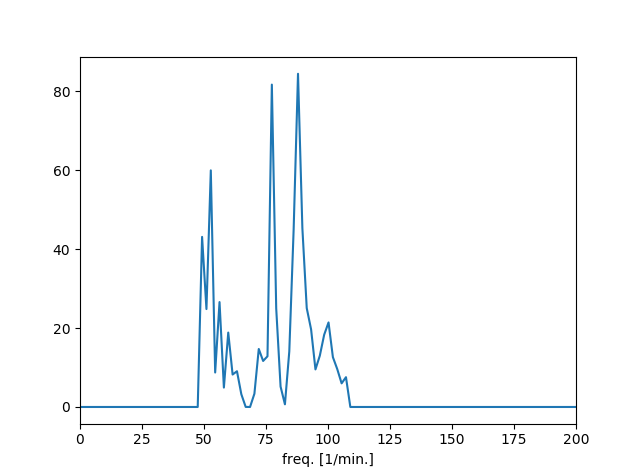
\includegraphics[width=8cm]{sample3-c200_200_5.png}
		\caption{Muestra 3: proximidad entre picos}
		\label{3prox1}
	\end{figure}
	
	\paragraph{} Tal como se ha observado en el método de promediado anterior, en la muestra 3, tras una inspección del gráfico de frecuencias, se observan dos picos de magnitud comparable. En este caso, el valor de la segunda frecuencia más representativa es de $77.419$, lo que representaría un $|Error| = 1.95\%$, el menor de todos los errores relativos obtenidos hasta el momento. 
	


	
	\newpage
	\begin{thebibliography}{9}
	

	
	\end{thebibliography}
	
\end{document}